\section{Introduction to R}
\frame{\sectionpage}

\begin{frame}{Getting and installing R}
  
  \begin{itemize}
  \item Available for Windows, Mac, Linux.
  \item Get R from \url{www.r-project.org}, install (standard way).
  \item Get R Studio from \url{www.rstudio.org}, install.
  \item R Studio is nicer-looking ``front end'' to R.
  \end{itemize}
  
\end{frame}

\begin{frame}[fragile]{Introduction to R}
  
  \begin{itemize}
  \item Start up R Studio.
  \item Look for Console Window (bottom left) with \texttt{>} prompt,
    click on window.
  \item Type R commands there, see output (\emph{not} point and
    click!). Eg:



    
\begin{knitrout}
\definecolor{shadecolor}{rgb}{0.969, 0.969, 0.969}\color{fgcolor}\begin{kframe}
\begin{alltt}
\hlstd{x}\hlkwb{=}\hlkwd{c}\hlstd{(}\hlnum{10}\hlstd{,}\hlnum{11}\hlstd{,}\hlnum{13}\hlstd{,}\hlnum{14}\hlstd{,}\hlnum{17}\hlstd{,}\hlnum{18}\hlstd{,}\hlnum{22}\hlstd{,}\hlnum{24}\hlstd{,}\hlnum{27}\hlstd{,}\hlnum{41}\hlstd{)}
\end{alltt}
\end{kframe}
\end{knitrout}
\item ``Glue those numbers into a ``list'' and save it in
  \texttt{x}'', \texttt{x} called a \textbf{variable}. To see what's
  in a variable, type its name:
  
  
 
\begin{knitrout}
\definecolor{shadecolor}{rgb}{0.969, 0.969, 0.969}\color{fgcolor}\begin{kframe}
\begin{alltt}
\hlstd{x}
\end{alltt}
\begin{verbatim}
##  [1] 10 11 13 14 17 18 22 24 27 41
\end{verbatim}
\end{kframe}
\end{knitrout}

\item Another variable and its value, ``5 through 37'':

{\small  
 
\begin{knitrout}
\definecolor{shadecolor}{rgb}{0.969, 0.969, 0.969}\color{fgcolor}\begin{kframe}
\begin{alltt}
\hlstd{z}\hlkwb{=}\hlnum{5}\hlopt{:}\hlnum{37}
\hlstd{z}
\end{alltt}
\begin{verbatim}
##  [1]  5  6  7  8  9 10 11 12 13 14 15 16
## [13] 17 18 19 20 21 22 23 24 25 26 27 28
## [25] 29 30 31 32 33 34 35 36 37
\end{verbatim}
\end{kframe}
\end{knitrout}
}  
  

  \end{itemize}
  
\end{frame}

\begin{frame}[fragile]{Statistics on variables}
  
  \begin{itemize}
  \item A ``summary'' of \texttt{x}:
 
\begin{knitrout}
\definecolor{shadecolor}{rgb}{0.969, 0.969, 0.969}\color{fgcolor}\begin{kframe}
\begin{alltt}
\hlkwd{summary}\hlstd{(x)}
\end{alltt}
\begin{verbatim}
##    Min. 1st Qu.  Median    Mean 3rd Qu. 
##   10.00   13.25   17.50   19.70   23.50 
##    Max. 
##   41.00
\end{verbatim}
\end{kframe}
\end{knitrout}

\begin{multicols}{2}

\item Or: mean:
\begin{knitrout}
\definecolor{shadecolor}{rgb}{0.969, 0.969, 0.969}\color{fgcolor}\begin{kframe}
\begin{alltt}
\hlkwd{mean}\hlstd{(x)}
\end{alltt}
\begin{verbatim}
## [1] 19.7
\end{verbatim}
\end{kframe}
\end{knitrout}

\item median:
  
 
\begin{knitrout}
\definecolor{shadecolor}{rgb}{0.969, 0.969, 0.969}\color{fgcolor}\begin{kframe}
\begin{alltt}
\hlkwd{median}\hlstd{(x)}
\end{alltt}
\begin{verbatim}
## [1] 17.5
\end{verbatim}
\end{kframe}
\end{knitrout}
  
\item standard deviation:
  
 
\begin{knitrout}
\definecolor{shadecolor}{rgb}{0.969, 0.969, 0.969}\color{fgcolor}\begin{kframe}
\begin{alltt}
\hlkwd{sd}\hlstd{(x)}
\end{alltt}
\begin{verbatim}
## [1] 9.357706
\end{verbatim}
\end{kframe}
\end{knitrout}

\item inter-quartile range (note UPPERCASE):
  
 
\begin{knitrout}
\definecolor{shadecolor}{rgb}{0.969, 0.969, 0.969}\color{fgcolor}\begin{kframe}
\begin{alltt}
\hlkwd{IQR}\hlstd{(x)}
\end{alltt}
\begin{verbatim}
## [1] 10.25
\end{verbatim}
\end{kframe}
\end{knitrout}
  
\end{multicols}
  
  

    
  \end{itemize}
  
\end{frame}


\begin{frame}[fragile]{Histogram}
  
\begin{knitrout}
\definecolor{shadecolor}{rgb}{0.969, 0.969, 0.969}\color{fgcolor}\begin{kframe}
\begin{alltt}
\hlkwd{hist}\hlstd{(x)}
\end{alltt}
\end{kframe}
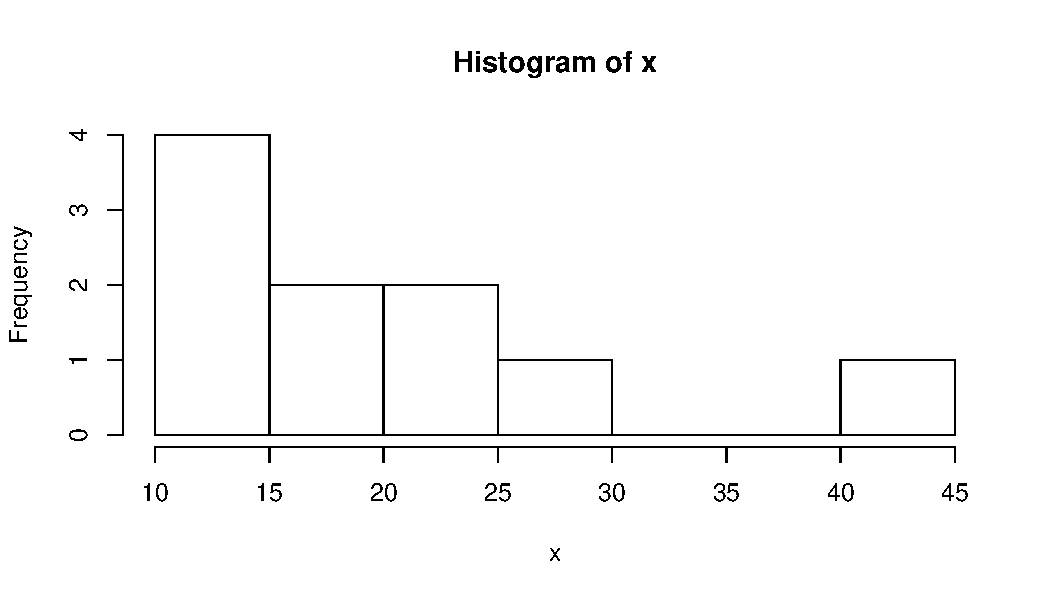
\includegraphics[width=\maxwidth]{figure/histo-1} 

\end{knitrout}
  
  
\end{frame}

\begin{frame}[fragile]{Better histogram}

  See \texttt{ggplot} section.
  
\begin{knitrout}
\definecolor{shadecolor}{rgb}{0.969, 0.969, 0.969}\color{fgcolor}\begin{kframe}
\begin{alltt}
\hlstd{d}\hlkwb{=}\hlkwd{data.frame}\hlstd{(x)}
\hlkwd{ggplot}\hlstd{(d,}\hlkwd{aes}\hlstd{(x))}\hlopt{+}\hlkwd{geom_histogram}\hlstd{(}\hlkwc{bins}\hlstd{=}\hlnum{7}\hlstd{)}
\end{alltt}
\end{kframe}
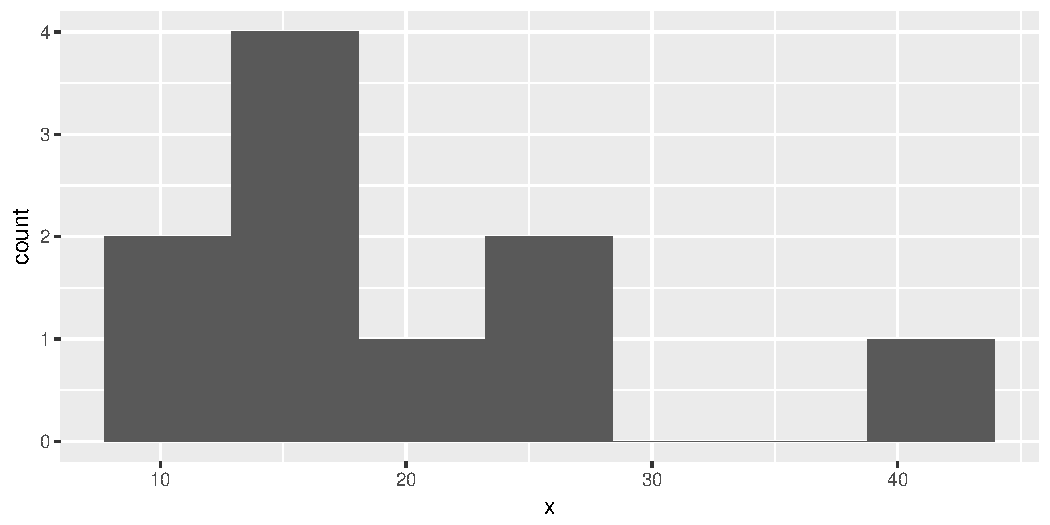
\includegraphics[width=\maxwidth]{figure/binsg-1} 

\end{knitrout}
  
\end{frame}

\begin{frame}[fragile]{Boxplot (comments next page)}
  
 
\begin{knitrout}
\definecolor{shadecolor}{rgb}{0.969, 0.969, 0.969}\color{fgcolor}\begin{kframe}
\begin{alltt}
\hlkwd{boxplot}\hlstd{(x)}
\end{alltt}
\end{kframe}
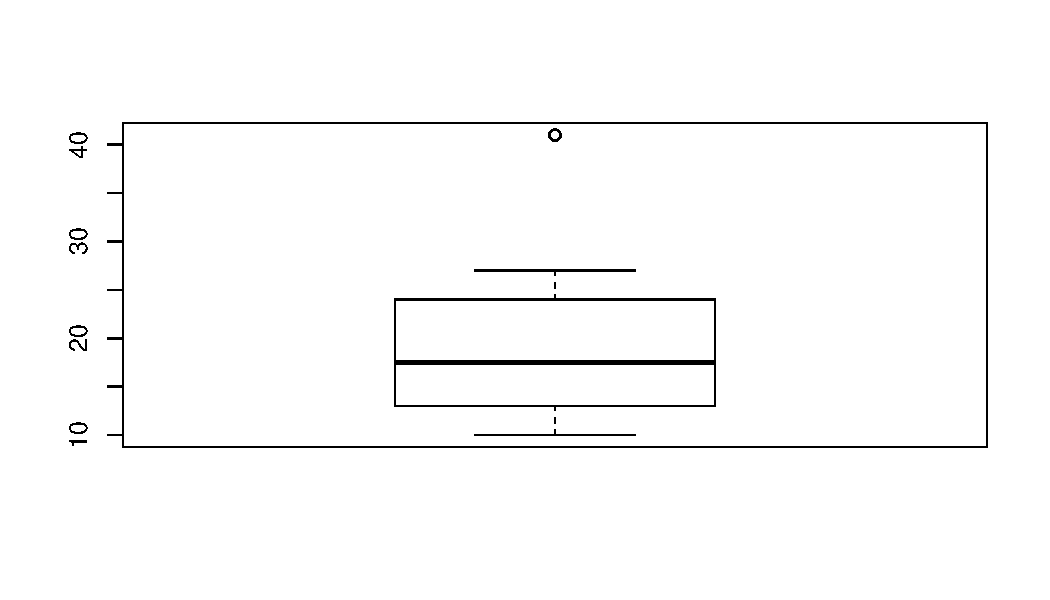
\includegraphics[width=\maxwidth]{figure/aslkhrliuf-1} 

\end{knitrout}
   
  
\end{frame}

\begin{frame}[fragile]{About the boxplot}
  
  \begin{itemize}
  \item Like histogram, shows centre, shape and spread of distribution.
  \item Based on median and quartiles.
  \item Middle of box is \textbf{median}.
  \item Top and bottom of  box are \textbf{quartiles}.
  \item Any values more than 1.5 times IQR below Q1 or above Q3
    considered \emph{outliers}, plotted separately.
  \item ``Whiskers'' join quartiles to most extreme data values.
  \end{itemize}
  
\end{frame}

\begin{frame}[fragile]{Reading data from text files}
  
  \begin{itemize}
  \item Text file like this, values separated by \emph{whitespace}:
\begin{verbatim}
xx yy   group
1  10   red
2   9   green
3  11   red
4  12   green
5  11   red
\end{verbatim}
  \item Saved in file \texttt{mydata.txt}. Read in via
    \texttt{read.table} and save in variable:
 
\begin{knitrout}
\definecolor{shadecolor}{rgb}{0.969, 0.969, 0.969}\color{fgcolor}\begin{kframe}
\begin{alltt}
\hlstd{my.data}\hlkwb{=}\hlkwd{read.table}\hlstd{(}\hlstr{"mydata.txt"}\hlstd{,}\hlkwc{header}\hlstd{=T)}
\hlstd{my.data}
\end{alltt}
\begin{verbatim}
##   xx yy group
## 1  1 10   red
## 2  2  9 green
## 3  3 11   red
## 4  4 12 green
## 5  5 11   red
\end{verbatim}
\end{kframe}
\end{knitrout}
    
  \end{itemize}
  
\end{frame}

\begin{frame}[fragile]{Getting the right folder}
  
  \begin{itemize}
  \item Sometimes R cannot find a data file.
  \item Set R's ``working directory'' to folder where data file is:
    \begin{itemize}
    \item In R Studio, select Session Menu, Set Working Directory,
      Choose Working Directory.
    \item Browse to folder where your data file is.
    \item Initially shows you what folder R is ``in''.
    \end{itemize}
  \end{itemize}
  
\end{frame}

\begin{frame}[fragile]{Data frame}
  
  \begin{itemize}
  \item \texttt{my.data} example of \textbf{data frame}: rows are
    observations, columns variables.
  \item \texttt{read.table} automatically creates data frame from text file.
  \item Columns by name:
 
\begin{knitrout}
\definecolor{shadecolor}{rgb}{0.969, 0.969, 0.969}\color{fgcolor}\begin{kframe}
\begin{alltt}
\hlstd{my.data}\hlopt{$}\hlstd{xx}
\end{alltt}
\begin{verbatim}
## [1] 1 2 3 4 5
\end{verbatim}
\begin{alltt}
\hlstd{my.data}\hlopt{$}\hlstd{group}
\end{alltt}
\begin{verbatim}
## [1] red   green red   green red  
## Levels: green red
\end{verbatim}
\end{kframe}
\end{knitrout}

\item Or, to save the \texttt{\$} stuff:
  
 
\begin{knitrout}
\definecolor{shadecolor}{rgb}{0.969, 0.969, 0.969}\color{fgcolor}\begin{kframe}
\begin{alltt}
\hlkwd{attach}\hlstd{(my.data)}
\hlstd{group}
\end{alltt}
\begin{verbatim}
## [1] red   green red   green red  
## Levels: green red
\end{verbatim}
\end{kframe}
\end{knitrout}
  

  \end{itemize}
  
\end{frame}

\begin{frame}[fragile]{Rows and columns by number}
  \begin{multicols}{2}
  \begin{itemize}

    
  \item \texttt{my.data}:
 
\begin{knitrout}
\definecolor{shadecolor}{rgb}{0.969, 0.969, 0.969}\color{fgcolor}\begin{kframe}
\begin{alltt}
\hlstd{my.data}
\end{alltt}
\begin{verbatim}
##   xx yy group
## 1  1 10   red
## 2  2  9 green
## 3  3 11   red
## 4  4 12 green
## 5  5 11   red
\end{verbatim}
\end{kframe}
\end{knitrout}
    
  \item The value in 3rd row and 2nd column:
 
\begin{knitrout}
\definecolor{shadecolor}{rgb}{0.969, 0.969, 0.969}\color{fgcolor}\begin{kframe}
\begin{alltt}
\hlstd{my.data[}\hlnum{3}\hlstd{,}\hlnum{2}\hlstd{]}
\end{alltt}
\begin{verbatim}
## [1] 11
\end{verbatim}
\end{kframe}
\end{knitrout}

\item Whole 3rd row:
 
\begin{knitrout}
\definecolor{shadecolor}{rgb}{0.969, 0.969, 0.969}\color{fgcolor}\begin{kframe}
\begin{alltt}
\hlstd{my.data[}\hlnum{3}\hlstd{,]}
\end{alltt}
\begin{verbatim}
##   xx yy group
## 3  3 11   red
\end{verbatim}
\end{kframe}
\end{knitrout}

\item Whole 2nd column:
  
 
\begin{knitrout}
\definecolor{shadecolor}{rgb}{0.969, 0.969, 0.969}\color{fgcolor}\begin{kframe}
\begin{alltt}
\hlstd{my.data[,}\hlnum{2}\hlstd{]}
\end{alltt}
\begin{verbatim}
## [1] 10  9 11 12 11
\end{verbatim}
\end{kframe}
\end{knitrout}

  
    
  \end{itemize}
    
  \end{multicols}
  
\end{frame}

\begin{frame}[fragile]{More selection}
  
  \begin{multicols}{2}
  \begin{itemize}
\item All the columns \emph{except} the second:
  
 
\begin{knitrout}
\definecolor{shadecolor}{rgb}{0.969, 0.969, 0.969}\color{fgcolor}\begin{kframe}
\begin{alltt}
\hlstd{my.data[,}\hlopt{-}\hlnum{2}\hlstd{]}
\end{alltt}
\begin{verbatim}
##   xx group
## 1  1   red
## 2  2 green
## 3  3   red
## 4  4 green
## 5  5   red
\end{verbatim}
\end{kframe}
\end{knitrout}

\item First through third rows:
  
 
\begin{knitrout}
\definecolor{shadecolor}{rgb}{0.969, 0.969, 0.969}\color{fgcolor}\begin{kframe}
\begin{alltt}
\hlstd{my.data[}\hlnum{1}\hlopt{:}\hlnum{3}\hlstd{,]}
\end{alltt}
\begin{verbatim}
##   xx yy group
## 1  1 10   red
## 2  2  9 green
## 3  3 11   red
\end{verbatim}
\end{kframe}
\end{knitrout}

\item Third and fifth rows:
  
 
\begin{knitrout}
\definecolor{shadecolor}{rgb}{0.969, 0.969, 0.969}\color{fgcolor}\begin{kframe}
\begin{alltt}
\hlstd{my.data[}\hlkwd{c}\hlstd{(}\hlnum{3}\hlstd{,}\hlnum{5}\hlstd{),]}
\end{alltt}
\begin{verbatim}
##   xx yy group
## 3  3 11   red
## 5  5 11   red
\end{verbatim}
\end{kframe}
\end{knitrout}
  

\end{itemize}
    
  \end{multicols}
  
\end{frame}


\begin{frame}[fragile]{Variable types}
  
  \begin{itemize}
  \item This:
 
\begin{knitrout}
\definecolor{shadecolor}{rgb}{0.969, 0.969, 0.969}\color{fgcolor}\begin{kframe}
\begin{alltt}
\hlstd{a}\hlkwb{=}\hlnum{2}
\hlstd{a}
\end{alltt}
\begin{verbatim}
## [1] 2
\end{verbatim}
\end{kframe}
\end{knitrout}
is a \textbf{scalar} (one value). 

\item This:
 
\begin{knitrout}
\definecolor{shadecolor}{rgb}{0.969, 0.969, 0.969}\color{fgcolor}\begin{kframe}
\begin{alltt}
\hlstd{x}
\end{alltt}
\begin{verbatim}
##  [1] 10 11 13 14 17 18 22 24 27 41
\end{verbatim}
\end{kframe}
\end{knitrout}
is a \textbf{vector} (several values).
\item This:
 
\begin{knitrout}
\definecolor{shadecolor}{rgb}{0.969, 0.969, 0.969}\color{fgcolor}\begin{kframe}
\begin{alltt}
\hlstd{group}
\end{alltt}
\begin{verbatim}
## [1] red   green red   green red  
## Levels: green red
\end{verbatim}
\end{kframe}
\end{knitrout}
is a \textbf{factor} (categorical/grouping variable).  

  \end{itemize}
  
\end{frame}

\begin{frame}[fragile]{Spreadsheet data}
  
  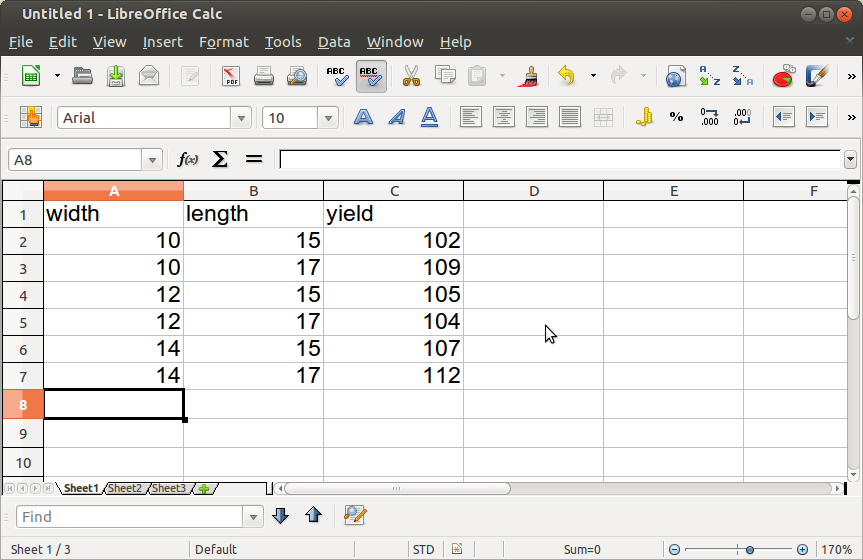
\includegraphics[width=4.5in]{myspread}
   
\end{frame}

\begin{frame}[fragile]{Reading into R}
  
  \begin{itemize}
  \item Save as \texttt{.csv} file (Text/CSV).
  \item Read in using \texttt{read.csv} (like \texttt{read.table}):
    
 
\begin{knitrout}
\definecolor{shadecolor}{rgb}{0.969, 0.969, 0.969}\color{fgcolor}\begin{kframe}
\begin{alltt}
\hlstd{tbl}\hlkwb{=}\hlkwd{read.csv}\hlstd{(}\hlstr{"myspread.csv"}\hlstd{,}\hlkwc{header}\hlstd{=T)}
\hlstd{tbl}
\end{alltt}
\begin{verbatim}
##   width length yield
## 1    10     15   102
## 2    10     17   109
## 3    12     15   105
## 4    12     17   104
## 5    14     15   107
## 6    14     17   112
\end{verbatim}
\end{kframe}
\end{knitrout}

\item Then use like any other data frame.
  \end{itemize}
  
\end{frame}
